% Options for packages loaded elsewhere
\PassOptionsToPackage{unicode}{hyperref}
\PassOptionsToPackage{hyphens}{url}
%
\documentclass[
]{article}
\usepackage{lmodern}
\usepackage{amsmath}
\usepackage{ifxetex,ifluatex}
\ifnum 0\ifxetex 1\fi\ifluatex 1\fi=0 % if pdftex
  \usepackage[T1]{fontenc}
  \usepackage[utf8]{inputenc}
  \usepackage{textcomp} % provide euro and other symbols
  \usepackage{amssymb}
\else % if luatex or xetex
  \usepackage{unicode-math}
  \defaultfontfeatures{Scale=MatchLowercase}
  \defaultfontfeatures[\rmfamily]{Ligatures=TeX,Scale=1}
\fi
% Use upquote if available, for straight quotes in verbatim environments
\IfFileExists{upquote.sty}{\usepackage{upquote}}{}
\IfFileExists{microtype.sty}{% use microtype if available
  \usepackage[]{microtype}
  \UseMicrotypeSet[protrusion]{basicmath} % disable protrusion for tt fonts
}{}
\makeatletter
\@ifundefined{KOMAClassName}{% if non-KOMA class
  \IfFileExists{parskip.sty}{%
    \usepackage{parskip}
  }{% else
    \setlength{\parindent}{0pt}
    \setlength{\parskip}{6pt plus 2pt minus 1pt}}
}{% if KOMA class
  \KOMAoptions{parskip=half}}
\makeatother
\usepackage{xcolor}
\IfFileExists{xurl.sty}{\usepackage{xurl}}{} % add URL line breaks if available
\IfFileExists{bookmark.sty}{\usepackage{bookmark}}{\usepackage{hyperref}}
\hypersetup{
  pdftitle={Gestion de Portefeuille},
  hidelinks,
  pdfcreator={LaTeX via pandoc}}
\urlstyle{same} % disable monospaced font for URLs
\usepackage[margin=1in]{geometry}
\usepackage{color}
\usepackage{fancyvrb}
\newcommand{\VerbBar}{|}
\newcommand{\VERB}{\Verb[commandchars=\\\{\}]}
\DefineVerbatimEnvironment{Highlighting}{Verbatim}{commandchars=\\\{\}}
% Add ',fontsize=\small' for more characters per line
\usepackage{framed}
\definecolor{shadecolor}{RGB}{248,248,248}
\newenvironment{Shaded}{\begin{snugshade}}{\end{snugshade}}
\newcommand{\AlertTok}[1]{\textcolor[rgb]{0.94,0.16,0.16}{#1}}
\newcommand{\AnnotationTok}[1]{\textcolor[rgb]{0.56,0.35,0.01}{\textbf{\textit{#1}}}}
\newcommand{\AttributeTok}[1]{\textcolor[rgb]{0.77,0.63,0.00}{#1}}
\newcommand{\BaseNTok}[1]{\textcolor[rgb]{0.00,0.00,0.81}{#1}}
\newcommand{\BuiltInTok}[1]{#1}
\newcommand{\CharTok}[1]{\textcolor[rgb]{0.31,0.60,0.02}{#1}}
\newcommand{\CommentTok}[1]{\textcolor[rgb]{0.56,0.35,0.01}{\textit{#1}}}
\newcommand{\CommentVarTok}[1]{\textcolor[rgb]{0.56,0.35,0.01}{\textbf{\textit{#1}}}}
\newcommand{\ConstantTok}[1]{\textcolor[rgb]{0.00,0.00,0.00}{#1}}
\newcommand{\ControlFlowTok}[1]{\textcolor[rgb]{0.13,0.29,0.53}{\textbf{#1}}}
\newcommand{\DataTypeTok}[1]{\textcolor[rgb]{0.13,0.29,0.53}{#1}}
\newcommand{\DecValTok}[1]{\textcolor[rgb]{0.00,0.00,0.81}{#1}}
\newcommand{\DocumentationTok}[1]{\textcolor[rgb]{0.56,0.35,0.01}{\textbf{\textit{#1}}}}
\newcommand{\ErrorTok}[1]{\textcolor[rgb]{0.64,0.00,0.00}{\textbf{#1}}}
\newcommand{\ExtensionTok}[1]{#1}
\newcommand{\FloatTok}[1]{\textcolor[rgb]{0.00,0.00,0.81}{#1}}
\newcommand{\FunctionTok}[1]{\textcolor[rgb]{0.00,0.00,0.00}{#1}}
\newcommand{\ImportTok}[1]{#1}
\newcommand{\InformationTok}[1]{\textcolor[rgb]{0.56,0.35,0.01}{\textbf{\textit{#1}}}}
\newcommand{\KeywordTok}[1]{\textcolor[rgb]{0.13,0.29,0.53}{\textbf{#1}}}
\newcommand{\NormalTok}[1]{#1}
\newcommand{\OperatorTok}[1]{\textcolor[rgb]{0.81,0.36,0.00}{\textbf{#1}}}
\newcommand{\OtherTok}[1]{\textcolor[rgb]{0.56,0.35,0.01}{#1}}
\newcommand{\PreprocessorTok}[1]{\textcolor[rgb]{0.56,0.35,0.01}{\textit{#1}}}
\newcommand{\RegionMarkerTok}[1]{#1}
\newcommand{\SpecialCharTok}[1]{\textcolor[rgb]{0.00,0.00,0.00}{#1}}
\newcommand{\SpecialStringTok}[1]{\textcolor[rgb]{0.31,0.60,0.02}{#1}}
\newcommand{\StringTok}[1]{\textcolor[rgb]{0.31,0.60,0.02}{#1}}
\newcommand{\VariableTok}[1]{\textcolor[rgb]{0.00,0.00,0.00}{#1}}
\newcommand{\VerbatimStringTok}[1]{\textcolor[rgb]{0.31,0.60,0.02}{#1}}
\newcommand{\WarningTok}[1]{\textcolor[rgb]{0.56,0.35,0.01}{\textbf{\textit{#1}}}}
\usepackage{graphicx}
\makeatletter
\def\maxwidth{\ifdim\Gin@nat@width>\linewidth\linewidth\else\Gin@nat@width\fi}
\def\maxheight{\ifdim\Gin@nat@height>\textheight\textheight\else\Gin@nat@height\fi}
\makeatother
% Scale images if necessary, so that they will not overflow the page
% margins by default, and it is still possible to overwrite the defaults
% using explicit options in \includegraphics[width, height, ...]{}
\setkeys{Gin}{width=\maxwidth,height=\maxheight,keepaspectratio}
% Set default figure placement to htbp
\makeatletter
\def\fps@figure{htbp}
\makeatother
\setlength{\emergencystretch}{3em} % prevent overfull lines
\providecommand{\tightlist}{%
  \setlength{\itemsep}{0pt}\setlength{\parskip}{0pt}}
\setcounter{secnumdepth}{-\maxdimen} % remove section numbering
\usepackage[utf8]{inputenc}
\usepackage{amsmath}
\usepackage{amsfonts}
\usepackage{amssymb}
\ifluatex
  \usepackage{selnolig}  % disable illegal ligatures
\fi

\title{Gestion de Portefeuille}
\usepackage{etoolbox}
\makeatletter
\providecommand{\subtitle}[1]{% add subtitle to \maketitle
  \apptocmd{\@title}{\par {\large #1 \par}}{}{}
}
\makeatother
\subtitle{TP-1: Analyse de l'indice CAC40}
\author{}
\date{\vspace{-2.5em}Version: 15 fév 2022}

\begin{document}
\maketitle

\begin{Shaded}
\begin{Highlighting}[]
\FunctionTok{library}\NormalTok{(lubridate)}
\FunctionTok{library}\NormalTok{(Hmisc)}
\FunctionTok{library}\NormalTok{(tseries)}
\FunctionTok{library}\NormalTok{(timeSeries)}


\NormalTok{get.src.folder }\OtherTok{\textless{}{-}} \ControlFlowTok{function}\NormalTok{() \{}
  \FunctionTok{path.expand}\NormalTok{(}\StringTok{"../GP/src"}\NormalTok{)}
\NormalTok{\}}

\NormalTok{get.data.folder }\OtherTok{\textless{}{-}} \ControlFlowTok{function}\NormalTok{() \{}
  \FunctionTok{path.expand}\NormalTok{(}\StringTok{"../GP/data"}\NormalTok{)}
\NormalTok{\}}

\FunctionTok{source}\NormalTok{(}\FunctionTok{file.path}\NormalTok{(}\FunctionTok{get.src.folder}\NormalTok{(), }\StringTok{\textquotesingle{}utils.R\textquotesingle{}}\NormalTok{))}
\end{Highlighting}
\end{Shaded}

\begin{verbatim}
## Warning: package 'spam' was built under R version 4.0.5
\end{verbatim}

\begin{Shaded}
\begin{Highlighting}[]
\FunctionTok{source}\NormalTok{(}\FunctionTok{file.path}\NormalTok{(}\FunctionTok{get.src.folder}\NormalTok{(), }\StringTok{\textquotesingle{}FileUtils.R\textquotesingle{}}\NormalTok{))}
\end{Highlighting}
\end{Shaded}

\hypertarget{les-donnuxe9es}{%
\subsection{Les données}\label{les-donnuxe9es}}

On charge les séries de rendements pour l'indice et les composants de
l'indice.

\begin{Shaded}
\begin{Highlighting}[]
\NormalTok{  ts.all }\OtherTok{\textless{}{-}} \FunctionTok{get.all.ts}\NormalTok{(}\StringTok{\textquotesingle{}CAC40\textquotesingle{}}\NormalTok{, }\AttributeTok{tickers=}\ConstantTok{NULL}\NormalTok{, }\AttributeTok{returns =} \ConstantTok{TRUE}\NormalTok{,}
    \AttributeTok{dt.start =} \FunctionTok{dmy}\NormalTok{(}\StringTok{\textquotesingle{}01Jul2007\textquotesingle{}}\NormalTok{), }\AttributeTok{combine =}\NormalTok{ T)}
  
  \CommentTok{\# bad data for Valeo}
\NormalTok{  ts.all }\OtherTok{\textless{}{-}}\NormalTok{ ts.all[,}\SpecialCharTok{{-}}\DecValTok{17}\NormalTok{]}
  
  \CommentTok{\# keep good data window}
\NormalTok{  ts.all }\OtherTok{\textless{}{-}} \FunctionTok{window}\NormalTok{(ts.all, }\FunctionTok{dmy}\NormalTok{(}\StringTok{\textquotesingle{}01Jul2007\textquotesingle{}}\NormalTok{), }
                   \FunctionTok{dmy}\NormalTok{(}\StringTok{\textquotesingle{}01Jan2009\textquotesingle{}}\NormalTok{))}
  
  \CommentTok{\# merge with cac40 index}
\NormalTok{  cac.index }\OtherTok{\textless{}{-}} \FunctionTok{get.ts}\NormalTok{(}\StringTok{\textquotesingle{}fchi\textquotesingle{}}\NormalTok{, }\StringTok{\textquotesingle{}CAC40\textquotesingle{}}\NormalTok{)}

\NormalTok{  cac.ret }\OtherTok{\textless{}{-}} \FunctionTok{returns}\NormalTok{(cac.index)}
  \FunctionTok{names}\NormalTok{(cac.ret) }\OtherTok{\textless{}{-}} \StringTok{\textquotesingle{}CAC40\textquotesingle{}}
\NormalTok{  ts.all }\OtherTok{\textless{}{-}} \FunctionTok{removeNA}\NormalTok{(}\FunctionTok{cbind}\NormalTok{(ts.all, cac.ret))}
\end{Highlighting}
\end{Shaded}

\begin{Shaded}
\begin{Highlighting}[]
\FunctionTok{plot}\NormalTok{(ts.all[, }\FunctionTok{c}\NormalTok{(}\DecValTok{1}\NormalTok{,}\DecValTok{2}\NormalTok{,}\DecValTok{3}\NormalTok{)], }\AttributeTok{main=}\StringTok{\textquotesingle{}Rendement quotidien\textquotesingle{}}\NormalTok{)}
\end{Highlighting}
\end{Shaded}

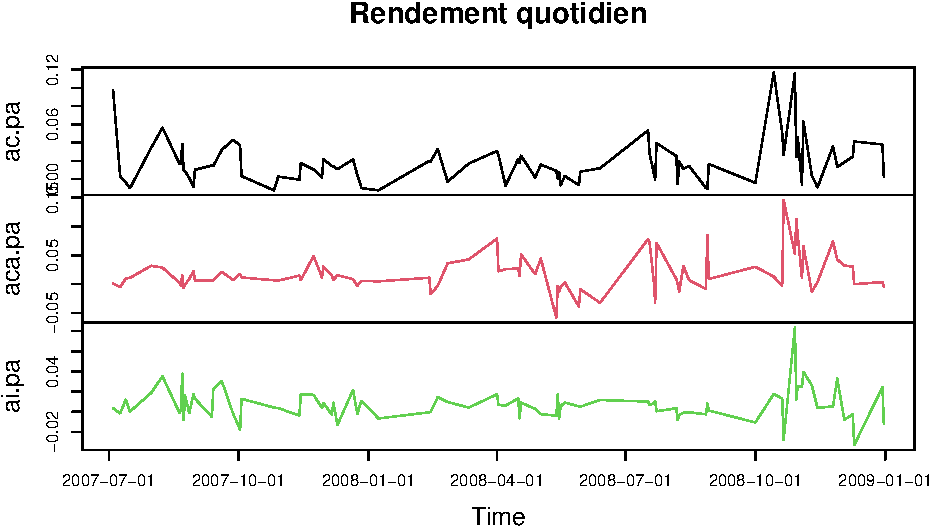
\includegraphics{TP1_files/figure-latex/plot-cac-1-1.pdf}

Puis on filtre les points suspects: rendements supérieur à 8 s.d.

\begin{Shaded}
\begin{Highlighting}[]
  \CommentTok{\# flag bad data points: \textgreater{} * \textbackslash{}sigma}
\NormalTok{  good.limit }\OtherTok{\textless{}{-}} \DecValTok{8}\SpecialCharTok{*}\FunctionTok{apply}\NormalTok{(ts.all, }\DecValTok{2}\NormalTok{, sd)}
  
\NormalTok{  ts.bad }\OtherTok{\textless{}{-}}\NormalTok{ ts.all}\SpecialCharTok{*}\ConstantTok{FALSE}
  \ControlFlowTok{for}\NormalTok{(j }\ControlFlowTok{in} \FunctionTok{seq}\NormalTok{(}\FunctionTok{ncol}\NormalTok{(ts.bad))) \{}
\NormalTok{    ts.bad[,j] }\OtherTok{\textless{}{-}} \FunctionTok{abs}\NormalTok{(ts.all[,j]) }\SpecialCharTok{\textgreater{}}\NormalTok{ good.limit[j]}
\NormalTok{  \}}
\NormalTok{  good.index }\OtherTok{\textless{}{-}} \SpecialCharTok{!}\FunctionTok{apply}\NormalTok{(ts.bad,}\DecValTok{1}\NormalTok{,any)}
\NormalTok{  ts.all }\OtherTok{\textless{}{-}}\NormalTok{ ts.all[good.index,]}
\end{Highlighting}
\end{Shaded}

Finalement, on calcule les rendements hebdomadaires:

\begin{Shaded}
\begin{Highlighting}[]
  \CommentTok{\# aggregate returns by week}
\NormalTok{  by }\OtherTok{\textless{}{-}} \FunctionTok{timeSequence}\NormalTok{(}\AttributeTok{from=}\FunctionTok{start}\NormalTok{(ts.all), }
                     \AttributeTok{to=}\FunctionTok{end}\NormalTok{(ts.all), }\AttributeTok{by=}\StringTok{\textquotesingle{}week\textquotesingle{}}\NormalTok{)}
\NormalTok{  ts.all.weekly }\OtherTok{\textless{}{-}} \FunctionTok{aggregate}\NormalTok{(ts.all, by, sum)}

\NormalTok{  ts.stocks }\OtherTok{\textless{}{-}}\NormalTok{ ts.all.weekly[,}\SpecialCharTok{{-}}\DecValTok{40}\NormalTok{]}
\NormalTok{  ts.index }\OtherTok{\textless{}{-}}\NormalTok{ ts.all.weekly[,}\DecValTok{40}\NormalTok{]}
\end{Highlighting}
\end{Shaded}

\begin{Shaded}
\begin{Highlighting}[]
\FunctionTok{plot}\NormalTok{(ts.index, }\AttributeTok{main=}\StringTok{\textquotesingle{}Rendement hebdomadaire de l}\SpecialCharTok{\textbackslash{}\textquotesingle{}}\StringTok{indice CAC40\textquotesingle{}}\NormalTok{)}
\end{Highlighting}
\end{Shaded}

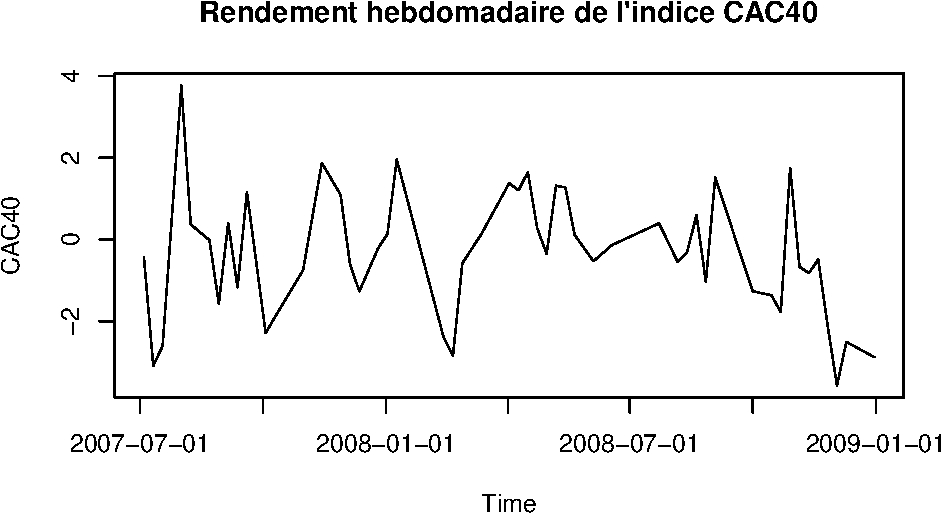
\includegraphics{TP1_files/figure-latex/plot-cac-2-1.pdf}

\hypertarget{calcul-de-correlation}{%
\subsection{Calcul de correlation}\label{calcul-de-correlation}}

\begin{itemize}
\item
  Calculer la matrice de corrélation des actions de l'indice.
\item
  Rechercher des actions fortement corrélées et d'autres qui semblent
  indépendantes. Justifier ces observations en considérant la nature des
  entreprises.
\item
  Choisir 3 titres, et reproduire la figure 3.5, page 35 du manuel de B.
  Pfaff. Commenter les résultats obtenus.
\end{itemize}

\hypertarget{analyse-en-composantes-principales}{%
\subsection{Analyse en composantes
principales}\label{analyse-en-composantes-principales}}

\begin{itemize}
\tightlist
\item
  Effectuer une ACP de la matrice de covariance des rendements
  hebdomadaires
\item
  Observer les projections des variables sur les premiers vecteurs
  propres, et tenter de fournir une interprétation économique de vos
  observations.
\end{itemize}

\end{document}
